\documentclass[a4paper, 11pt]{article}
\usepackage{comment} 
\usepackage{fullpage} 
\usepackage[spanish]{babel} 
\selectlanguage{spanish}
\usepackage[utf8]{inputenc}
\usepackage{float} 
\usepackage{graphicx}
\usepackage{ marvosym }
\usepackage{amsthm}
\usepackage{amsmath}
\usepackage[sort&compress, numbers]{natbib}
\usepackage{amssymb}
\usepackage{hyperref}
%\hypersetup{colorlinks=True, citecolor=blue}
\hypersetup{colorlinks=true, citecolor=green, urlcolor=blue}

\begin{document}
\begin{center}
\LARGE \bf Pr\'actica 12\\ Red neuronal
\end{center}

\vspace{1cm} 
\noindent\textbf {Edson Edgardo Samaniego Pantoja} \hfill \textbf{Materia:} Simulación computacional 
\hfill \\
\textbf{Fecha} \today  
\vspace{1cm} 

\section{Introducción}
Esta última práctica consiste en la demostración básica de aprendizaje a máquina que consiste en reconocer dígitos de imágenes pequeñas en blanco y negro con una red neuronal.
Un elemento básico de esta red es el perceptron que es un hiper plano que busca
colocarse en la frontera que separa entradas verdaderas y las entradas falsas.
Para la práctica es dado un código en el repositorio de Schaeffer \cite{elisa} que es mejor explicado paso a paso en su pagina web \cite{dra}, consiste en que el perceptron diga falso cuando la imagen es un cero y verdadero cuando la imagen contiene un uno, pero se extiende esta idea a los diez dígitos de cero a nueve. Lo que significa que se asocian los números a vectores de largo fijo de verdades y falsos, lo que se logra fácilmente con sus representaciones en números binarios.

Además de codificar las respuestas deseadas, se realiza el poder generar entradas que no sean todas idénticas para que haya algo de reto en obtener la respuesta correcta. Se crean imágenes de dígitos de una manera probabilística a partir de plantillas. Los píxeles que son negros en la plantilla serán puestas casi siempre, mientras los grises ocasionalmente, y los blancos solamente como ruido aleatorio de poca frecuencia.

\section{Objetivo}
Estudiar de manera sistemática el desempeño de la red neuronal en términos de su puntaje F (F-score) para los diez dígitos en función de las tres probabilidades asignadas a la generación de los dígitos (ngb), variando a las tres en un experimento factorial adecuado.

\section{Código}
Lo primero que se realiza en el código de Samaniego \cite{Edson} es la forma en que se varian de manera dispersa en valores de \texttt{n,g,b} para poder observar qué factor es con el que mejor trabaja la red neuronal. Para eso se genera un dispersión en un gráfico de tres dimensiones para que cada punto represente el valor de \texttt{x,y,z} respectivamente a \texttt{n,g,b}. Se puede observar en figura \ref{f1}.
\begin{figure}[H]
  \centering      
  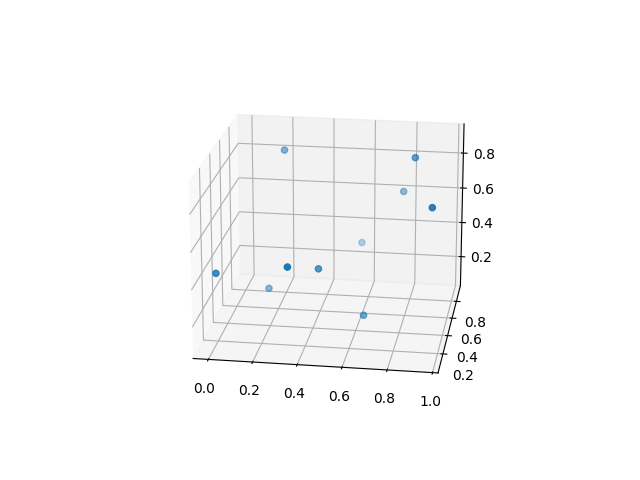
\includegraphics[scale=.8]{3d.png}
  \caption{Gráfico de dispersión tres dimensiones para valores de \texttt{n,g,b}.}
  \label{f1}
\end{figure}

\begin{verbatim}
from pyDOE import lhs
var=3
muestras =10
x= lhs(var, muestras, criterion="corr")
fig = plt.figure()
ax = fig.add_subplot(111, projection='3d')
ax.scatter(x[:,0], x[:,1], x[:,2])
plt.show()

\end{verbatim}

Después se entra a un ciclo que varía cada punto de la dispersión o cada coordenada de tres dígitos y se extrae la posición de valor para \texttt{n,g,b} respectivamente. En la variable modelos donde se asignan los valores ya mencionados simplemente se remplazo por la variable que estará cambiando en cada ciclo.

\begin{verbatim}
for ciclos in range(0, muestras):

    posiciones= x[ciclos]
    posn=posiciones[0]
    posg=posiciones[1]
    posb=posiciones[2]
    modelos = pd.read_csv('digits.txt', sep=' ', header = None)
    modelos = modelos.replace({'n': posn, 'g': posg, 'b': posb})
    r, c = 5, 3
    dim = r * c
    tasa = 0.15
    tranqui = 0.99
    tope = 9

\end{verbatim}

En cada ciclo una vez que termina el entrenamiento y la prueba, se extrae de la matriz de confusión generada el \texttt{F-score} para los datos.
Obteniendo como final en la variable \texttt{precision} interpretada como porcentaje de qué tanto mejora el resultado reconociendo imágenes de números, con los valores dados en un inicio de \texttt{n,g,b}.

\begin{verbatim}
    contadores2=np.delete(contadores,10,1)# elimina la columna 10
    TP= np.diag(contadores2)
    FP= np.sum(contadores2, axis=0)-TP
    FN = np.sum(contadores2, axis=1) - TP  
    num_classes = 10
    TN = []
    for i in range(num_classes):
        temp = np.delete(contadores2, i, 0)
        temp = np.delete(temp, i, 1)  
        TN.append(sum(sum(temp)))
    
    precision= TP/(TP+FP)    
    
\end{verbatim}


\section{Resultados}
Los resultados pueden revisarse en la siguiente tabla \ref{tab1} donde se puede ver para cada muestra que valores de negro gris y blanco se dieron y como afecto estos datos al reconocimiento de la red neuronal y viendo que mejora se ve según la condición.


\begin{table}[H]
        \caption{Registro por muestra, valores de n,g,b y sus promedios resultantes en reconocimiento de dígitos.}
        \bigskip
        \label{tab1}
        \centering
        \begin{tabular}{|r|r|r|r|}
        \hline
         Muestra&valor \texttt{n,g,b}&Promedio&Promedio (TP)  \\
        \hline
        1 & 0.62, 0.45, 0.08 & 0.19 & 4.3 \\
        \hline
        2 & 0.54, 0.93, 0.28 & 0.18 & 4.3 \\
        \hline
        3 & 0.00, 0.17, 0.41 & 0.11 & 2.7 \\
        \hline
        4 & 0.34, 0.06, 0.52 & 0.16 & 3.7 \\
        \hline
        5 & 0.20, 0.73, 0.87 & 0.24 & 6.6 \\
        \hline
        6 & 0.43, 0.34, 0.39 & 0.09 & 2.7 \\
        \hline
        7 & 0.16, 0.57, 0.15 & 0.14 & 3.0 \\
        \hline
        8 & 0.76, 0.83, 0.63 & 0.11 & 3.1 \\
        \hline
        9 & 0.83, 0.62, 0.90 & 0.09 & 2.7 \\
        \hline
        10 & 0.95, 0.29, 0.77 & 0.21 & 5.0 \\
        \hline
        
        \end{tabular}
    \end{table}

\bigskip
Los resultados de la tabla se pueden ver gráficamente en los diagramas caja bigote de la figura \ref{f2} realizados donde cada uno representa los datos obtenidos de la variable \texttt{precision} la cual tiene el porcentaje de efectividad en reconocimiento de cada número.

\begin{figure}[H]
  \centering      
  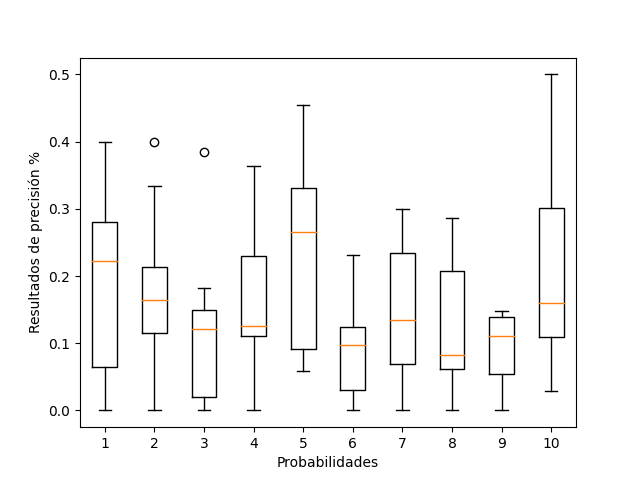
\includegraphics[scale=.8]{boxplot1.png}
  \caption{Caja bigote por cada muestra realizada y sus datos expresados en porcentaje de efectividad en el reconocimiento de números.}
  \label{f2}
\end{figure}

\begin{figure}[H]
  \centering      
  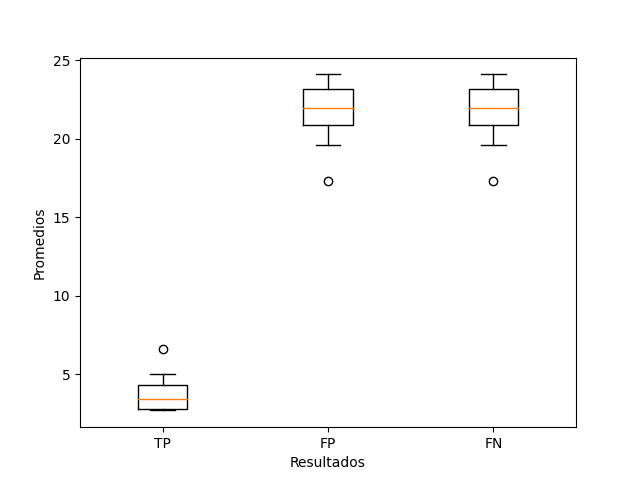
\includegraphics[scale=.8]{boxplot2.png}
  \caption{Caja bigote de los promedios que se obtienen de TP, FP, y FN.}
  \label{f3}
\end{figure}


\section{Conclusión}

En base a la tabla \ref{tab1} y figura \ref{f2} se puede concluir en que la mejor combinación de negro, gris y blanco se da cuando la probabilidad de blanco y gris es mas grande o mas probable que la de negro ya que se vuelve mas flexible la manera de reconocimiento de los números dados.
El porcentaje mas bajo se obtiene cuando la probabilidad de negro es mas alta que las otras dos pero gris y blanco se encuentran muy cercanos en sus probabilidades.

\bibliography{refe}
\bibliographystyle{plainnat}

\end{document}
